\documentclass{article}
\usepackage[final]{nips_2017}
\usepackage[polish]{babel}
\usepackage[utf8]{inputenc} % allow utf-8 input
\usepackage[T1]{fontenc}    % use 8-bit T1 fonts
\usepackage{hyperref}       % hyperlinks
\usepackage{url}            % simple URL typesetting
\usepackage{booktabs}       % professional-quality tables
\usepackage{amsfonts}       % blackboard math symbols
\usepackage{nicefrac}       % compact symbols for 1/2, etc.
\usepackage{microtype}      % microtypography
\usepackage{graphicx}
\usepackage[section]{placeins}
\graphicspath{ {./images/} }

\title{ Sieć konwolucyjna  }

\author{
  Autor: Rafał Behrendt \\
  \texttt{246643@student.pwr.edu.pl} \\
  Prowadząca: dr hab. inż. Urszula Markowska-Kaczmar \\
  \today
}

\begin{document}

\maketitle

\begin{abstract}
  Celem ćwiczenia jest zapoznanie się działaniem sieci z warstwami konwolucyjnymi. Eksperymenty przeprowadzono na zbiorze
  MNIST zawierającym 60000 danych treningowych oraz 10000 danych testowych.
\end{abstract}

Kod źródłowy znajduje się w poniższym linku:

\begin{center}
  \url{https://github.com/aspirew/neuralNetworks/tree/list4}
\end{center}

\newpage
\section{Eksperymenty}

Za domyślne hiperparametry przyjęto:

\begin{itemize}
  \item Ilość warstw konwolucyjnych: 2
  \item Ilość warstw w pełni połączonych: 2 (1 warstwa ukryta o rozmiarze 128 neuronów i warstwa wyjściowa)
  \item Wielkość kernela: (3, 3)
  \item Wielkości map cech: 32, 64
  \item Współczynnik uczenia: 0.01
  \item Inicjalizacja wag: metoda xaviera
  \item Optymalizator: Adam
  \item Funkcja straty: Entropia krzyżowa
  \item Funkcja aktywacji: ReLU
\end{itemize}

Każdy test przeszedł przez 10 epok zanim został zakończony.
Aby zbadać prędkość nauki przyjęto wartość progową $0.98$ dokładności i sprawdzono, po ilu epokach wartość ta jest osiągana.
Wartość ta określona jest w tabelach w kolumnie z nagłówkiem \textbf{wytrenowanie}

\section{Porównanie wydajności sieci MLP i sieci z jedną warstwą konwolucyjną}

Został przeprowadzony eksperyment porównujący wydajność sieci MLP bez warstw konwolucyjnych z siecią wielowarstwową z jedną warstwą konwolucyjną.
Sieć MLP posiadała dwie warstwy ukryte o rozmiarach 128 i 64 neurony. Po każdej warstwie zastosowano dropout. W drugiej sieci znajdowała się jedna warstwa
konwolucyjna i domyślne warstwy w pełni połączone.

\subsection{Sieć MLP}

\begin{table}[h]
  \centering
    
  \bgroup
  \def\arraystretch{1.3}
\begin{tabular}{|l|l|l|l|l|l|}
\hline
Epoka & Czas wykonania [s] & Błąd & Dokładność & Błąd dev & Dokładność dev \\ \hline
1 & 3 & 0.376 & 0.8865 & 0.1567 & 0.9517 \\ \hline
2 & 2 & 0.2022 & 0.9404 & 0.1353 & 0.9588 \\ \hline
3 & 2 & 0.1734 &  0.9489 & 0.1281 & 0.9608 \\ \hline
4 & 2 & 0.151 &  0.954 & 0.1284 & 0.9660 \\ \hline
5 & 2 & 0.1417 & 0.9577 & 0.1153 & 0.9693 \\ \hline
6 & 2 & 0.1263 & 0.9615 & 0.1220 & 0.9689 \\ \hline
7 & 2 & 0.1196 & 0.9645 & 0.1162 & 0.9692 \\ \hline
8 & 2 & 0.1108 & 0.9664 & 0.1212 & 0.9695 \\ \hline
9 & 2 & 0.1208 & 0.9645 & 0.1252 & 0.9676 \\ \hline
10 & 2 & 0.1062 & 0.9683 & 0.1145 & 0.9712 \\ \hline
\end{tabular}
  \egroup
  \vspace{10pt}
  \caption{Wyniki wykonania sieci MLP}
\end{table}

Błąd na zbiorze testowym: $0.1127$ \newline
Dokładność na zbiorze testowym: $0.9717$

Sieć osiąga bardzo dobre wyniki nawet bez warstw konwolucyjnych.

\newpage
\begin{figure}[h]
  \centering
  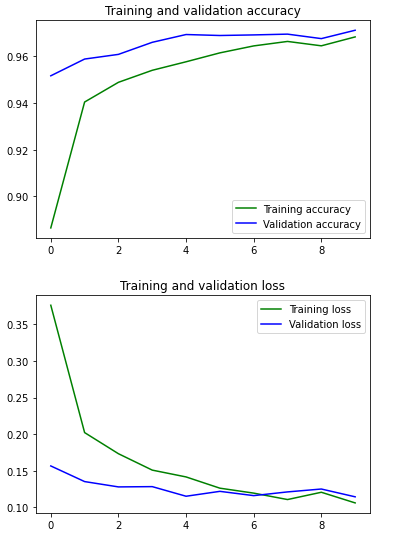
\includegraphics[width=\linewidth]{mlp.png}
\end{figure}

\newpage
\subsection{Sieć z warstwą konwolucyjną}

\begin{table}[!htb]
  \centering
    
  \bgroup
  \def\arraystretch{1.3}
\begin{tabular}{|l|l|l|l|l|l|}
\hline
Epoka & Czas wykonania [s] & Błąd & Dokładność & Błąd dev & Dokładność dev \\ \hline
1 & 11 & 0.2364 & 0.9289 & 0.0902 & 0.9729 \\ \hline
2 & 11 & 0.0865 & 0.9729 & 0.0680 & 0.9807 \\ \hline
3 & 11 & 0.0649 & 0.9793 & 0.0691 & 0.9787 \\ \hline
4 & 11 & 0.0511 & 0.9837 & 0.0678 & 0.9817 \\ \hline
5 & 11 & 0.0462 & 0.9849 & 0.0755 & 0.9812 \\ \hline
6 & 11 & 0.0393 & 0.9870 & 0.0746 & 0.9814 \\ \hline
7 & 11 & 0.0380 & 0.9872 & 0.0789 & 0.9813 \\ \hline
8 & 11 & 0.0288 & 0.9902 & 0.0866 & 0.9816 \\ \hline
9 & 10 & 0.0309 & 0.9902 & 0.0859 & 0.9825 \\ \hline
10 & 11 & 0.0317 & 0.9896 & 0.0936 & 0.9797 \\ \hline
\end{tabular}
  \egroup
  \vspace{10pt}
  \caption{Wyniki wykonania sieci MLP}
\end{table}

Błąd na zbiorze testowym: $0.0682$ \newline
Dokładność na zbiorze testowym: $0.9829$

Sieć osiąga lepsze wyniki, ale to na co należy przede wszystkim zwórcić uwagę to fakt, sieć uczy się dużo szybciej i już po 3 epoce osiąga
moment w którym zaczyna się przeuczać, na co wskazuje zwiększająca się wartość błędu dla zbioru walidacyjnego. Sieć MLP po 10 epokach wciąż poprawia swoje działanie.
Z drugiej strony sieć MLP pod względem wydajnościowym jest niemal 3 razy szybsza, co też należy wziąć pod uwagę.

\newpage
\begin{figure}[h]
  \centering
  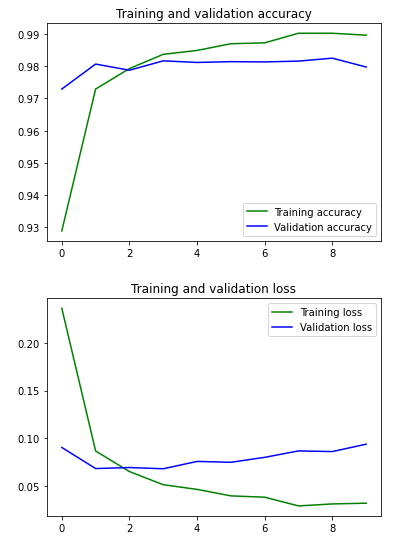
\includegraphics[width=\linewidth]{conv_compare.png}
\end{figure}

\newpage
\section{Test ilości warstw konwolucyjnych z warstwami poolingu}

Zbadano jak ilość warstw konwolucyjnych wpływa na skuteczność sieci. Zastosowano kernel wielkości (3, 3), 
za wielkość ramki odpowiadał wykorzytany framework keras, ilość map cech wynosiła w pierwszej warstwie 32 i z każdą warstwą zwiększała się dwukrotnie.
Po każdej warstwie zastosowano warstwę poolingu.
Przedstawione w tabelce wyniki odnoszą się do wyników sieci na zbiorze testowym. Wykresy odnoszą się do wyników sieci na zbiorze treningowym i walidacyjnym.

\begin{table}[h]
  \centering
    
  \bgroup
  \def\arraystretch{1.3}
\begin{tabular}{|l|l|l|l|l|}
\hline
Ilość warstw konwolucyjnych & Czas trenowania [s] & Wytrenowanie [epoka] & Błąd & Skuteczność \\ \hline
3 & 220 & 1 & 0.0524 & 0.9876 \\ \hline
2 & 170 & 1 & 0.0772 & 0.9850 \\ \hline
1 & 90 & 1 & 0.1102 & 0.9810 \\ \hline
\end{tabular}
  \egroup
  \vspace{10pt}
  \caption{Zastosowanie różnej ilosci warstw konwolucyjnych}
\end{table}

\begin{figure}[h]
  \centering
  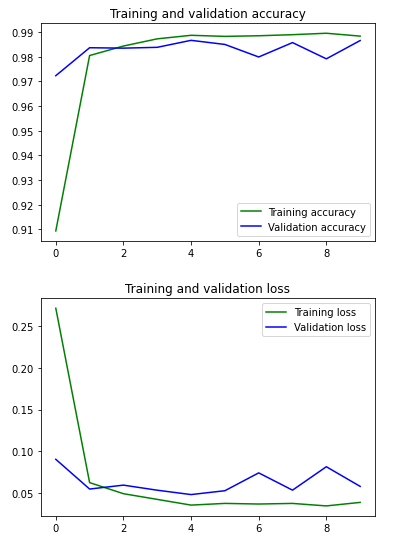
\includegraphics[width=\linewidth]{3_conv_3_max.png}
  \caption{3 warstwy konwolucyje z 3 warstwami poolingu}
\end{figure}

\begin{figure}[h]
  \centering
  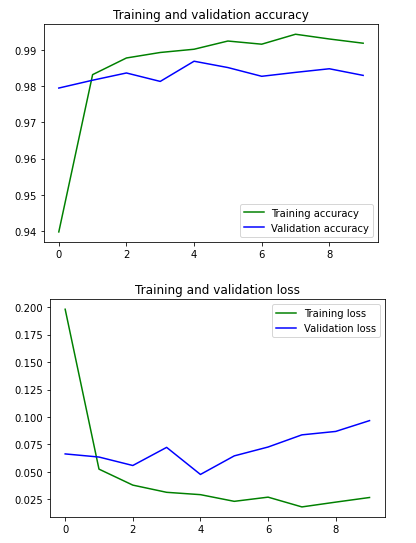
\includegraphics[width=\linewidth]{2_conv_2_max.png}
  \caption{2 warstwy konwolucyje z 2 warstwami poolingu}
\end{figure}

\begin{figure}[h]
  \centering
  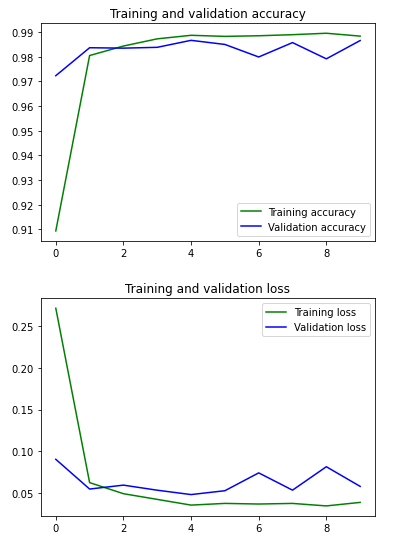
\includegraphics[width=\linewidth]{3_conv_3_max.png}
  \caption{1 warstwa konwolucyje z 1 warstwaą poolingu}
\end{figure}

Wraz ze wzrostem ilości warstw konwolucyjnych rośnie dokładność wyników uczenia. Można jednak zauważyć też,
że wyniki zbioru walidacyjnego coraz bardziej odbiegają od wyników na zbiorze trenującym co może świadczyć
przeuczeniu sieci.


\section{Test ilości warstw konwolucyjnych bez warstw poolingu}

Powtórzono poprzednie badanie bez wykorzystania warstw poolingu.

\begin{table}[h]
  \centering
    
  \bgroup
  \def\arraystretch{1.3}
\begin{tabular}{|l|l|l|l|l|}
\hline
Ilość warstw konwolucyjnych & Czas trenowania [s] & Wytrenowanie [epoka] & Błąd & Skuteczność \\ \hline
3 & 1421 & 2 & 0.088 & 0.98 \\ \hline
2 & 497 & 2 & 0.0788 & 0.9831 \\ \hline
1 & 111 & 2 & 0.1156 & 0.9782 \\ \hline
\end{tabular}
  \egroup
  \vspace{10pt}
  \caption{Zastosowanie różnej ilosci warstw konwolucyjnych bez warstw poolingu}
\end{table}

\begin{figure}[!htb]
  \centering
  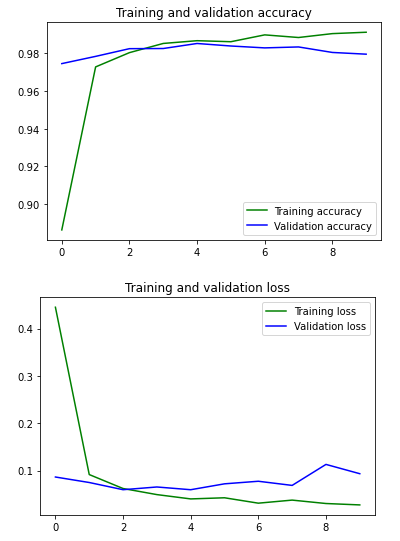
\includegraphics[width=\linewidth]{3_conv.png}
  \caption{3 warstwy konwolucyje z 3 warstwami poolingu}
\end{figure}

\begin{figure}[!htb]
  \centering
  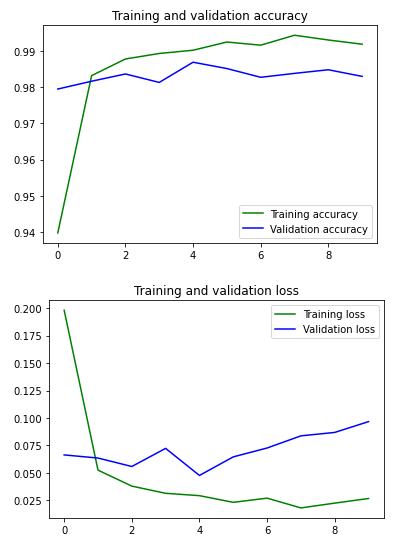
\includegraphics[width=\linewidth]{2_conv.png}
  \caption{2 warstwy konwolucyje z 2 warstwami poolingu}
\end{figure}

\begin{figure}[!htb]
  \centering
  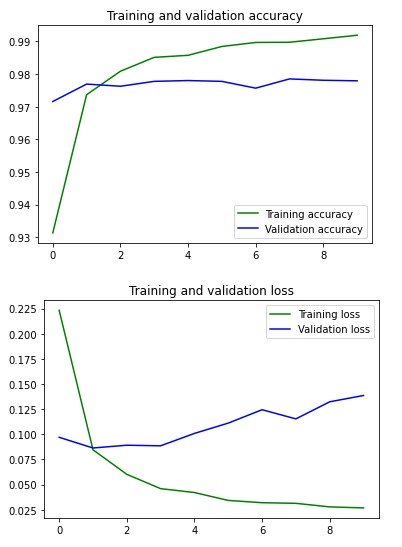
\includegraphics[width=\linewidth]{1_conv.png}
  \caption{1 warstwa konwolucyje z 1 warstwą poolingu}
\end{figure}

Można zauważyć dużą różnicę w porównaniu z poprzednim eksperymentem. Zastosowanie poolingu ma na celu
zmniejszenie wielkosci obrazu, czym samym zmniejszamy ilość koniecznych obliczeń, a także ignorujemy nieistotne
dla terningu cechy. Jak można zauważyć za dużo szczegółów branych pod uwagę znacząco wydłuża wykonanie sieci pod względem
wydajnościowym jak i pod względem prędkości zmiany błędu. Ostateczne wyniki skuteczności nie odbiegają od eksperymentu z wykorzystaniem warstw poolingu,
są nawet nieco gorsze.

\newpage
\section{Test wielkości kernela}

Zbadano jak wielkość kernela wpływa na skuteczność i prędkosć nauki sieci. Badanie przeprowadzono na jednej warstwie konwolucyjnej.
Przedstawione w tabelce wyniki odnoszą się do wyników sieci na zbiorze testowym. Wykresy odnoszą się do wyników sieci na zbiorze treningowym i walidacyjnym.

\begin{table}[h]
  \centering
    
  \bgroup
  \def\arraystretch{1.3}
\begin{tabular}{|l|l|l|l|l|}
\hline
Wielkość kernela & Czas trenowania [s] & Osiągnięcie progu [epoka] & Błąd & Skuteczność \\ \hline
(2, 2) & 84 & 4 & 0.0873 & 0.9801 \\ \hline
(3, 3) & 108 & 2 & 0.0764 & 0.9811 \\ \hline
(5, 5) & 122 & 3 & 0.0744 & 0.9850 \\ \hline
(7, 7) & 147 & 3 & 0.0744 & 0.9810 \\ \hline
(11, 11) & 220 & 4 & 0.0864 & 0.9818 \\ \hline
\end{tabular}
  \egroup
  \vspace{10pt}
  \caption{Zastosowanie różnej wielkości kernela}
\end{table}

\begin{figure}[h]
  \centering
  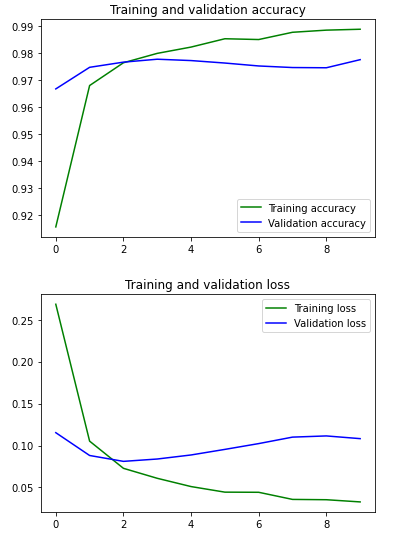
\includegraphics[width=\linewidth]{kernel_2_2.png}
  \caption{Kernel wielkości 2x2}
\end{figure}

\begin{figure}[h]
  \centering
  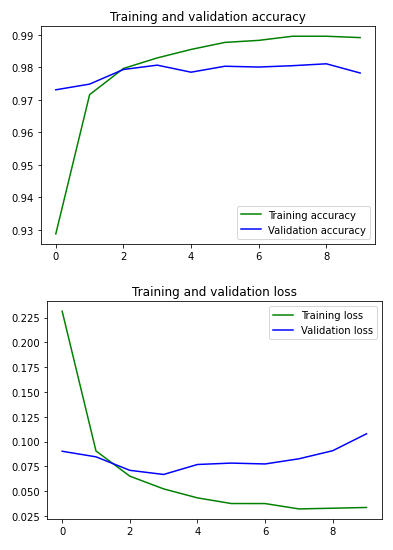
\includegraphics[width=\linewidth]{kernel_3_3.png}
  \caption{Kernel wielkości 3x3}
\end{figure}

\begin{figure}[h]
  \centering
  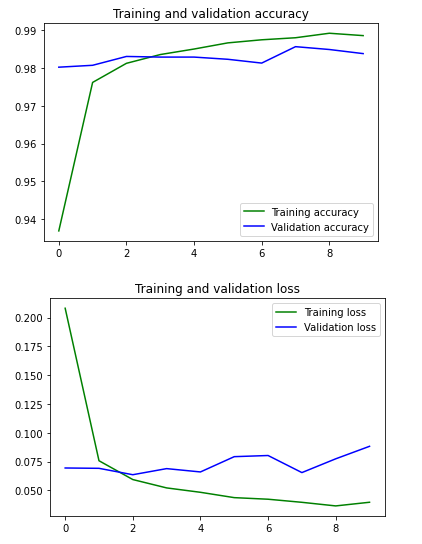
\includegraphics[width=\linewidth]{kernel_5_5.png}
  \caption{Kernel wielkości 5x5}
\end{figure}

\begin{figure}[h]
  \centering
  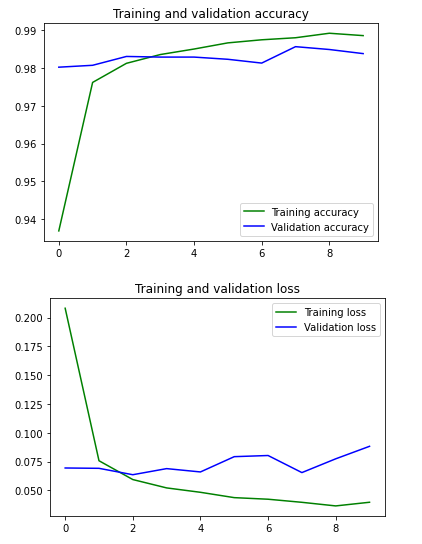
\includegraphics[width=\linewidth]{kernel_7_7.png}
  \caption{Kernel wielkości 7x7}
\end{figure}


\begin{figure}[h]
  \centering
  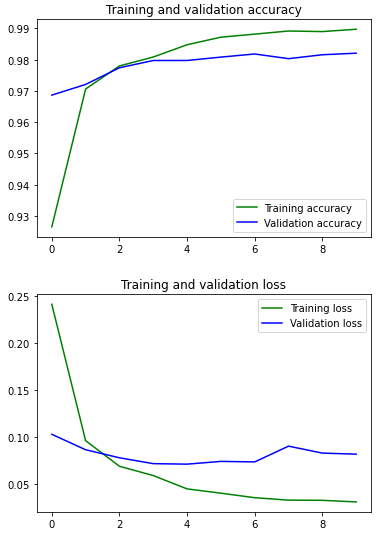
\includegraphics[width=\linewidth]{kernel_11_11.png}
  \caption{Kernel wielkości 11x11}
\end{figure}

Można zauważyć że dopasowanie wielkości kernela ma znaczenie dla skuteczności sieci. Zbyt niski kernel może okazać się za mały aby zauważyć daną istotną cechę.
Zbyt duży z kolei może brać pod uwagę zbyt ogólny obszar obrazu, czym samym przeoczyć cechy które faktycznie są istotne.
Dobór wielkości kernela powinien zależeć od wielkości obrazu. Dla problemu w tym zadaniu, można zauważyć, że dla wielkości kernela 3 sieć uczy się najszybciej.
Nie widać znaczącej różnicy w skuteczności. Ponadto wraz ze wzrostem kernela, rośnie czas obliczeń, ponieważ sieć ma więcej wag do dopasowania.

\newpage
\section{Test wielkości mapy cech}

Zbadano jak wielkość mapy cech wpływa na skuteczność i prędkość nauki sieci.
Przedstawione w tabelce wyniki odnoszą się do wyników sieci na zbiorze testowym. Wykresy odnoszą się do wyników sieci na zbiorze treningowym i walidacyjnym.

\begin{table}[h]
  \centering
    
  \bgroup
  \def\arraystretch{1.3}
\begin{tabular}{|l|l|l|l|l|}
\hline
Wielkość mapy cech & Czas trenowania [s] & Osiągnięcie progu [epoka] & Błąd & Skuteczność \\ \hline
32 & 101 & 3 & 0.0878 & 0.9835 \\ \hline
64 & 189 & 3 & 0.0901 & 0.981 \\ \hline
128 & 343 & 3 & 0.0943 & 0.9793 \\ \hline
256 & 679 & 4 & 0.0878 & 0.9822 \\ \hline
\end{tabular}
  \egroup
  \vspace{10pt}
  \caption{Zastosowanie różnej wielkości mapy cech}
\end{table}

\begin{figure}[!htb]
  \centering
  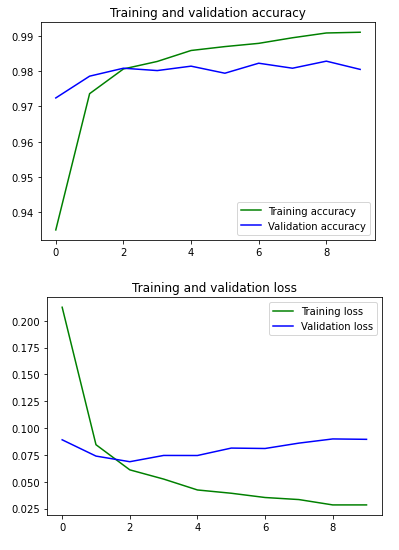
\includegraphics[width=\linewidth]{feature_32.png}
  \caption{Warstwa konwolucyjna z mapą cech o wielkości 32}
\end{figure}

\begin{figure}[!htb]
  \centering
  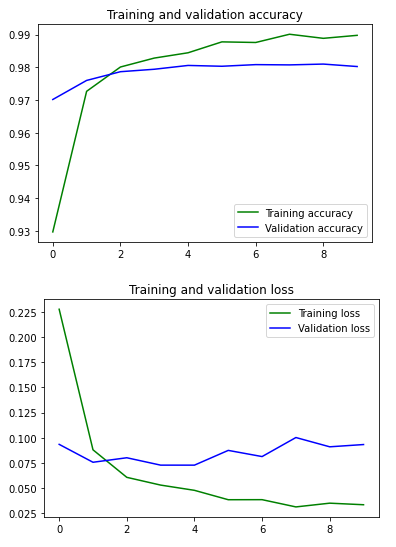
\includegraphics[width=\linewidth]{feature_64.png}
  \caption{Warstwa konwolucyjna z mapą cech o wielkości 64}
\end{figure}

\begin{figure}[!htb]
  \centering
  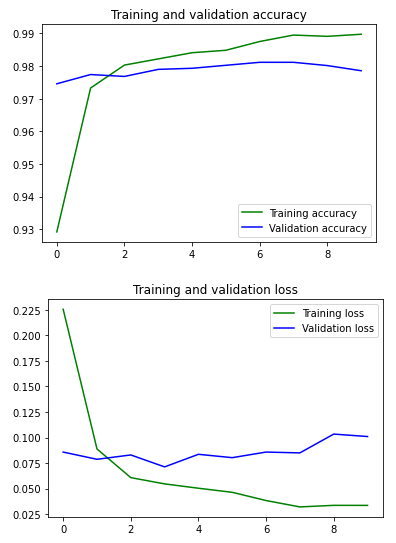
\includegraphics[width=\linewidth]{feature_128.png}
  \caption{Warstwa konwolucyjna z mapą cech o wielkości 128}
\end{figure}

\begin{figure}[!htb]
  \centering
  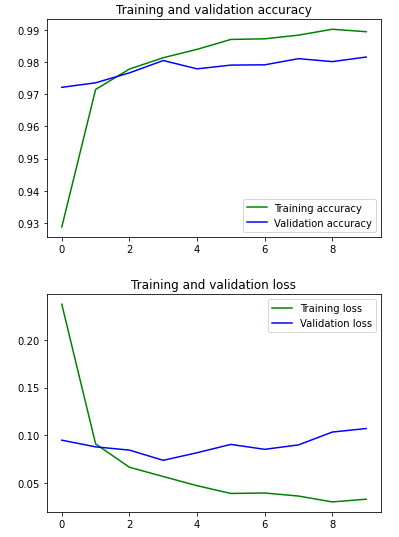
\includegraphics[width=\linewidth]{feature_256.png}
  \caption{Warstwa konwolucyjna z mapą cech o wielkości 256}
\end{figure}

Wielkość mapy cech mówi o tym, jak wiele charakterystycznych cech sieć będzie rozpoznawać na obrazie. 
Zbyt duża ilość może doprowadzić do przeuczenia sieci, co widoczne jest na wykresach - błąd zbioru walidacyjnego sukcesywnie rośnie.
Im więcej map cech tym więcej obliczeń do wykonania, zatem czas wykonania rośnie.

\section{Testy poolingu}

Zbadano jak wielkość i metoda poolingu wpływa na prędkość nauki i skuteczność sieci.

\subsection{Average pooling}

\begin{table}[h]
  \centering
    
  \bgroup
  \def\arraystretch{1.3}
\begin{tabular}{|l|l|l|l|l|}
\hline
Wielkość poolingu & Czas trenowania [s] & Osiągnięcie progu [epoka] & Błąd & Skuteczność \\ \hline
2x2 & 86 & 4 & 0.0776 & 0.9825 \\ \hline
3x3 & 77 & 3 & 0.0682 & 0.981 \\ \hline
5x5 & 75 & 7 & 0.0530 & 0.9836 \\ \hline
10x10 & 70 & - & 0.1010 & 0.9623 \\ \hline
\end{tabular}
  \egroup
  \vspace{10pt}
  \caption{Zastosowanie różnej wielkości mapy cech}
\end{table}

\begin{figure}[h]
  \centering
  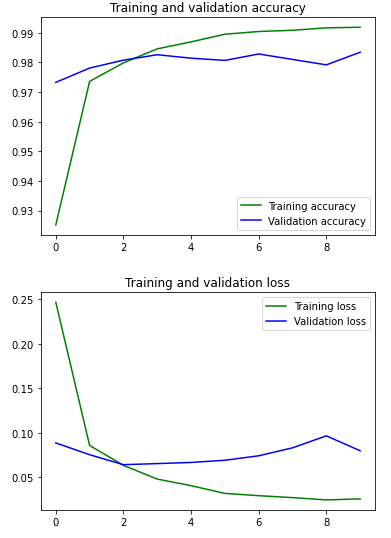
\includegraphics[width=\linewidth]{pooling_2_2.png}
  \caption{Average pooling o wielkości 2x2}
\end{figure}

\begin{figure}[h]
  \centering
  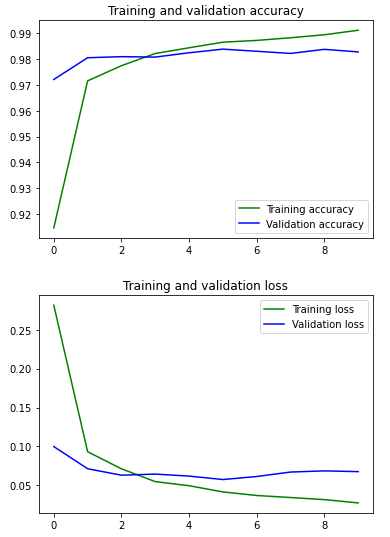
\includegraphics[width=\linewidth]{pooling_3_3.png}
  \caption{Average pooling o wielkości 3x3}
\end{figure}

\begin{figure}[h]
  \centering
  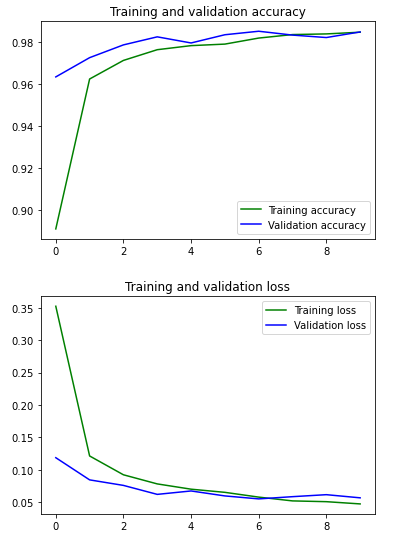
\includegraphics[width=\linewidth]{pooling_5_5.png}
  \caption{Average pooling o wielkości 5x5}
\end{figure}

\begin{figure}[h]
  \centering
  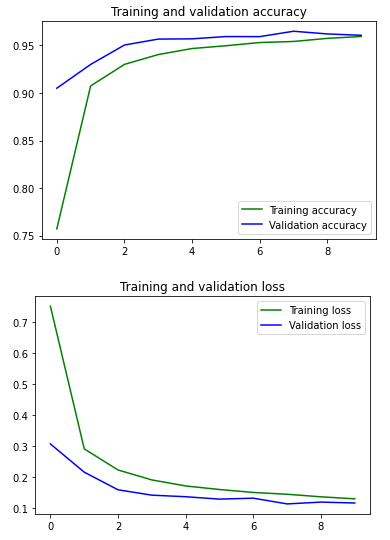
\includegraphics[width=\linewidth]{pooling_10_10.png}
  \caption{Average pooling o wielkości 10x10}
\end{figure}

\subsection{Max pooling}

\begin{table}[h]
  \centering
    
  \bgroup
  \def\arraystretch{1.3}
\begin{tabular}{|l|l|l|l|l|}
\hline
Wielkość poolingu & Czas trenowania [s] & Osiągnięcie progu [epoka] & Błąd & Skuteczność \\ \hline
2x2 & 87 & 4 & 0.0965 & 0.9796 \\ \hline
3x3 & 76 & 2 & 0.0727 & 0.9803 \\ \hline
5x5 & 70 & 4 & 0.0646 & 0.9823 \\ \hline
10x10 & 66 & - & 0.1155 & 0.9639 \\ \hline
\end{tabular}
  \egroup
  \vspace{10pt}
  \caption{Zastosowanie różnej wielkości mapy cech}
\end{table}

\begin{figure}[!htb]
  \centering
  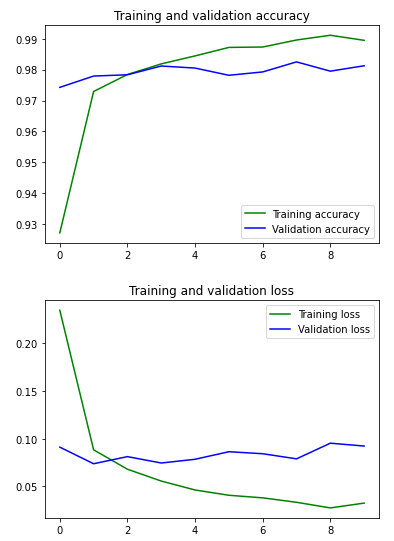
\includegraphics[width=\linewidth]{pooling_max_2_2.png}
  \caption{Max pooling o wielkości 2x2}
\end{figure}

\begin{figure}[!htb]
  \centering
  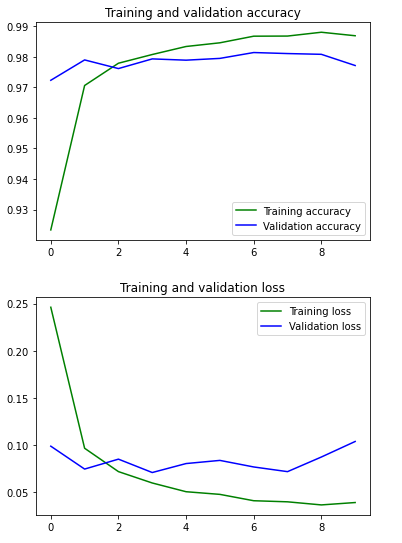
\includegraphics[width=\linewidth]{pooling_max_3_3.png}
  \caption{Max pooling o wielkości 3x3}
\end{figure}

\begin{figure}[!htb]
  \centering
  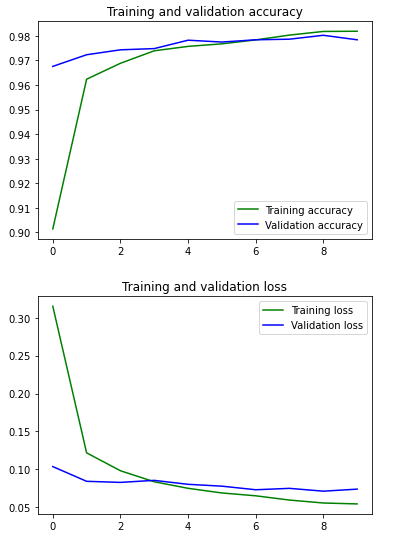
\includegraphics[width=\linewidth]{pooling_max_5_5.png}
  \caption{Max pooling o wielkości 5x5}
\end{figure}

\begin{figure}[!htb]
  \centering
  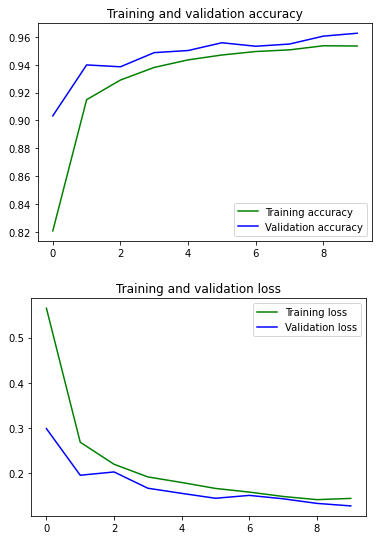
\includegraphics[width=\linewidth]{pooling_max_10_10.png}
  \caption{Max pooling o wielkości 10x10}
\end{figure}

Widać że wraz ze wzrostem wielkości poolingu rośnie nieznacznie prędkość wykonania kodu, jednakże zauważalny jest duży spadek
prędkości nauki sieci.

Różnica pomiędy Average poolingiem i Max poolingiem nie jest zauważalna. Z reguły stosowany jest Max pooling.

\section{Podsumowanie}

Warstwy konwolucyjne mogą przycznić się do znacznego usprawnienia działania sieci. Eksperymenty wykazały, że sieć konwolucyjna
radzi sobie lepiej ze zbiorem MNIST niż robiła to sieć bez warstw konwolucyjnych. Do tak prostego problemu wykorzystałbym jednak
zwykłą sieć bez warstw konwolucyjnych - ze względu na znacznie większą prędkość obliczeń bez dużej straty na skuteczności sieci.
Sieć konwolucyjna znacznie lepiej poradzi sobie przy bardziej złożonych problemach jak rozpoznawnie obiektów (także w kolorze), rozpoznawanie
twarzy, itp.

\end{document}